\begin{savequote}[75mm]
The feeling is less like an ending than just another starting point.
\qauthor{Chuck Palahniuk}
\end{savequote}

\chapter{Combined Run 1 $H\rightarrow WW^{*}\rightarrow \ell\nu\ell\nu$ results}

\section{Introduction}

In the final statistical analysis of \HWWfull, the dedicated gluon-gluon fusion and vector boson fusion sensitive signal regions are all combined into a single fit to determine the main parameters of interest, the Higgs signal strength $\mu$ and mass $m_H$. Therefore, while the specific requirements applied for the VBF sensitive analysis are discussed in chapter 5, the final measurement of these parameters can only be discussed in combination with the results of the ggF dedicated analysis. For example, because ggF Higgs production is considered a background in the VBF analysis, the ggF dedicated signal regions can actually constrain the normalization of this background in the VBF dedicated region.

This chapter presents the combined interpretation of results in the \HWWfull analysis for gluon fusion and vector boson fusion Higgs production. First, the results of the dedicated gluon fusion search are presented. Then, a comparison of the individual production mode signal strengths ($\mu_{\ggF}$ and $\mu_{\VBF}$ and a measurement of the combined signal strength ($\mu$) are shown. Subsequently, the measured values of the Higgs couplings to fermions and vector bosons is presented. Finally, the cross section measurement for ggF and VBF production are shown. 

\section{Results of dedication gluon fusion \HWWfull search}

The details of the dedicated gluon fusion \HWWfull search are not discussed in this thesis and instead left to more comprehensive sources\cite{WW2015}. However, a brief summary of the results are essential for describing the results of the full analysis and interpreting the results of the dedicated VBF search in this broader context. 

Table~\ref{tab:fitregions} shows the individual signal regions that were input into the final statistical fit. The ggF dedicated bins use $\mTH$ as their discriminating variable and are separated into bins of $\pT$ of the subleading lepton as well. The VBF dedicated bin uses the $\bdt$ distribution as its final discriminant. 

\begin{table*}[tb!]
\centering%
\captionsetup{justification=centering}

%--------------------------------------------------------------------------------
\begin{tabular*}{\textwidth}{
  p{0.3\textwidth}
  l %p{0.100\textwidth}
  l %p{0.100\textwidth}
  l
  c
  c
}
\\
\dbline
\multicolumn{4}{c}{SR category $i$}
&
&\multicolumn{1}{l}{\multirow{2}{*}{Fit var.}}
\\
\clineskip%
\cline{1-4}%
\clineskip%
$\Njet$, flavor
&${\otimes\,}\mll$
&${\otimes\,}\pTsublead$
&${\otimes\,}\ell_2$
&
&
\\
\sgline
$\NjetEQzero$ \\
\quad $\DFchan$     &${\otimes\,}[10,30,55]$ &${\otimes\,}[10,15,20,\infty]$ &${\otimes\,}[e,\mu]$ &&$\mTH$ \\
\quad $\SFchan$     &${\otimes\,}[12,55]$    &${\otimes\,}[10,\infty]$       &                     &&$\mTH$ \\
\sgline
$\NjetEQone$ \\
\quad $\DFchan$     &${\otimes\,}[10,30,55]$ &${\otimes\,}[10,15,20,\infty]$ &${\otimes\,}[e,\mu]$ &&$\mTH$ \\
\quad $\SFchan$     &${\otimes\,}[12,55]$    &${\otimes\,}[10,\infty]$       &                     &&$\mTH$ \\
\sgline
$\NjetGEtwo$ ggF \\
\quad $\DFchan$     &${\otimes\,}[10,55]$    &${\otimes\,}[10,\infty]$       &                     &&$\mTH$ \\
\sgline
\multicolumn{2}{l}{$\NjetGEtwo$ VBF} \\
\quad $\DFchan$     &${\otimes\,}[10,50]$    &${\otimes\,}[10,\infty]$       &                     &&$\bdt$ \\
\quad $\SFchan$     &${\otimes\,}[12,50]$    &${\otimes\,}[10,\infty]$       &                     &&$\bdt$ \\
\end{tabular*}
\caption{
  All signal regions definitions input into final statistical fit\cite{WW2015}.
}
\label{tab:fitregions}
\end{table*}
%eof

Table~\ref{tab:final-yields} shows the yields in the various signal regions in both data and expected signal and backgrounds. The yields for signal and background are all scaled according to the final normalizations calculated in the fit. 


\begin{table}[h!]
\centering
\captionsetup{justification=centering}

%\begin{tabular*}{0.480\textwidth}{p{0.075\textwidth} p{0.180\textwidth} l}
\hspace{-10pt}
\begin{tabular}{|c|c|c|c|c|}
\hline
 & $N_{\rm obs}$ & $N_{\rm bkg}$ & $N_{\rm ggF}$ & $N_{\rm VBF}$ \\ \hline
$\Njet = 0$ & $3750$ & $3430 \pm 90$ & $300 \pm 50$ & $8 \pm 4$ \\ \hline
$\Njet = 1$ & $1596$ & $1470 \pm 40$ & $102 \pm 26$ & $17 \pm 5$ \\ \hline
$\Njet \geq 2$, $\rm ggF$ $e\mu$ & $1017$ & $960 \pm 40$ & $37 \pm 11$ & $13 \pm 1.4$ \\ \hline
$\Njet \geq 2$, $\rm VBF$ & $130$ & $99 \pm 9$ & $7.7 \pm 2.6$ & $21 \pm 3$ \\ \hline
\end{tabular}

\caption{
Post-fit yields in the different ggF and VBF dedicated signal regions\cite{WW2015}. 
}
\label{tab:final-yields}
\end{table}

Figure~\ref{fig:ggF-mT} shows the final post-fit $\mTH$ distribution in the $\Njet \leq 1$ regions. The data are very consistent with the hypothesis of ggF Higgs production. 

\begin{figure}[h!]
  %\vspace{20pt}
  \centering
  \captionsetup{justification=centering}

  %\hspace*{-32pt}
  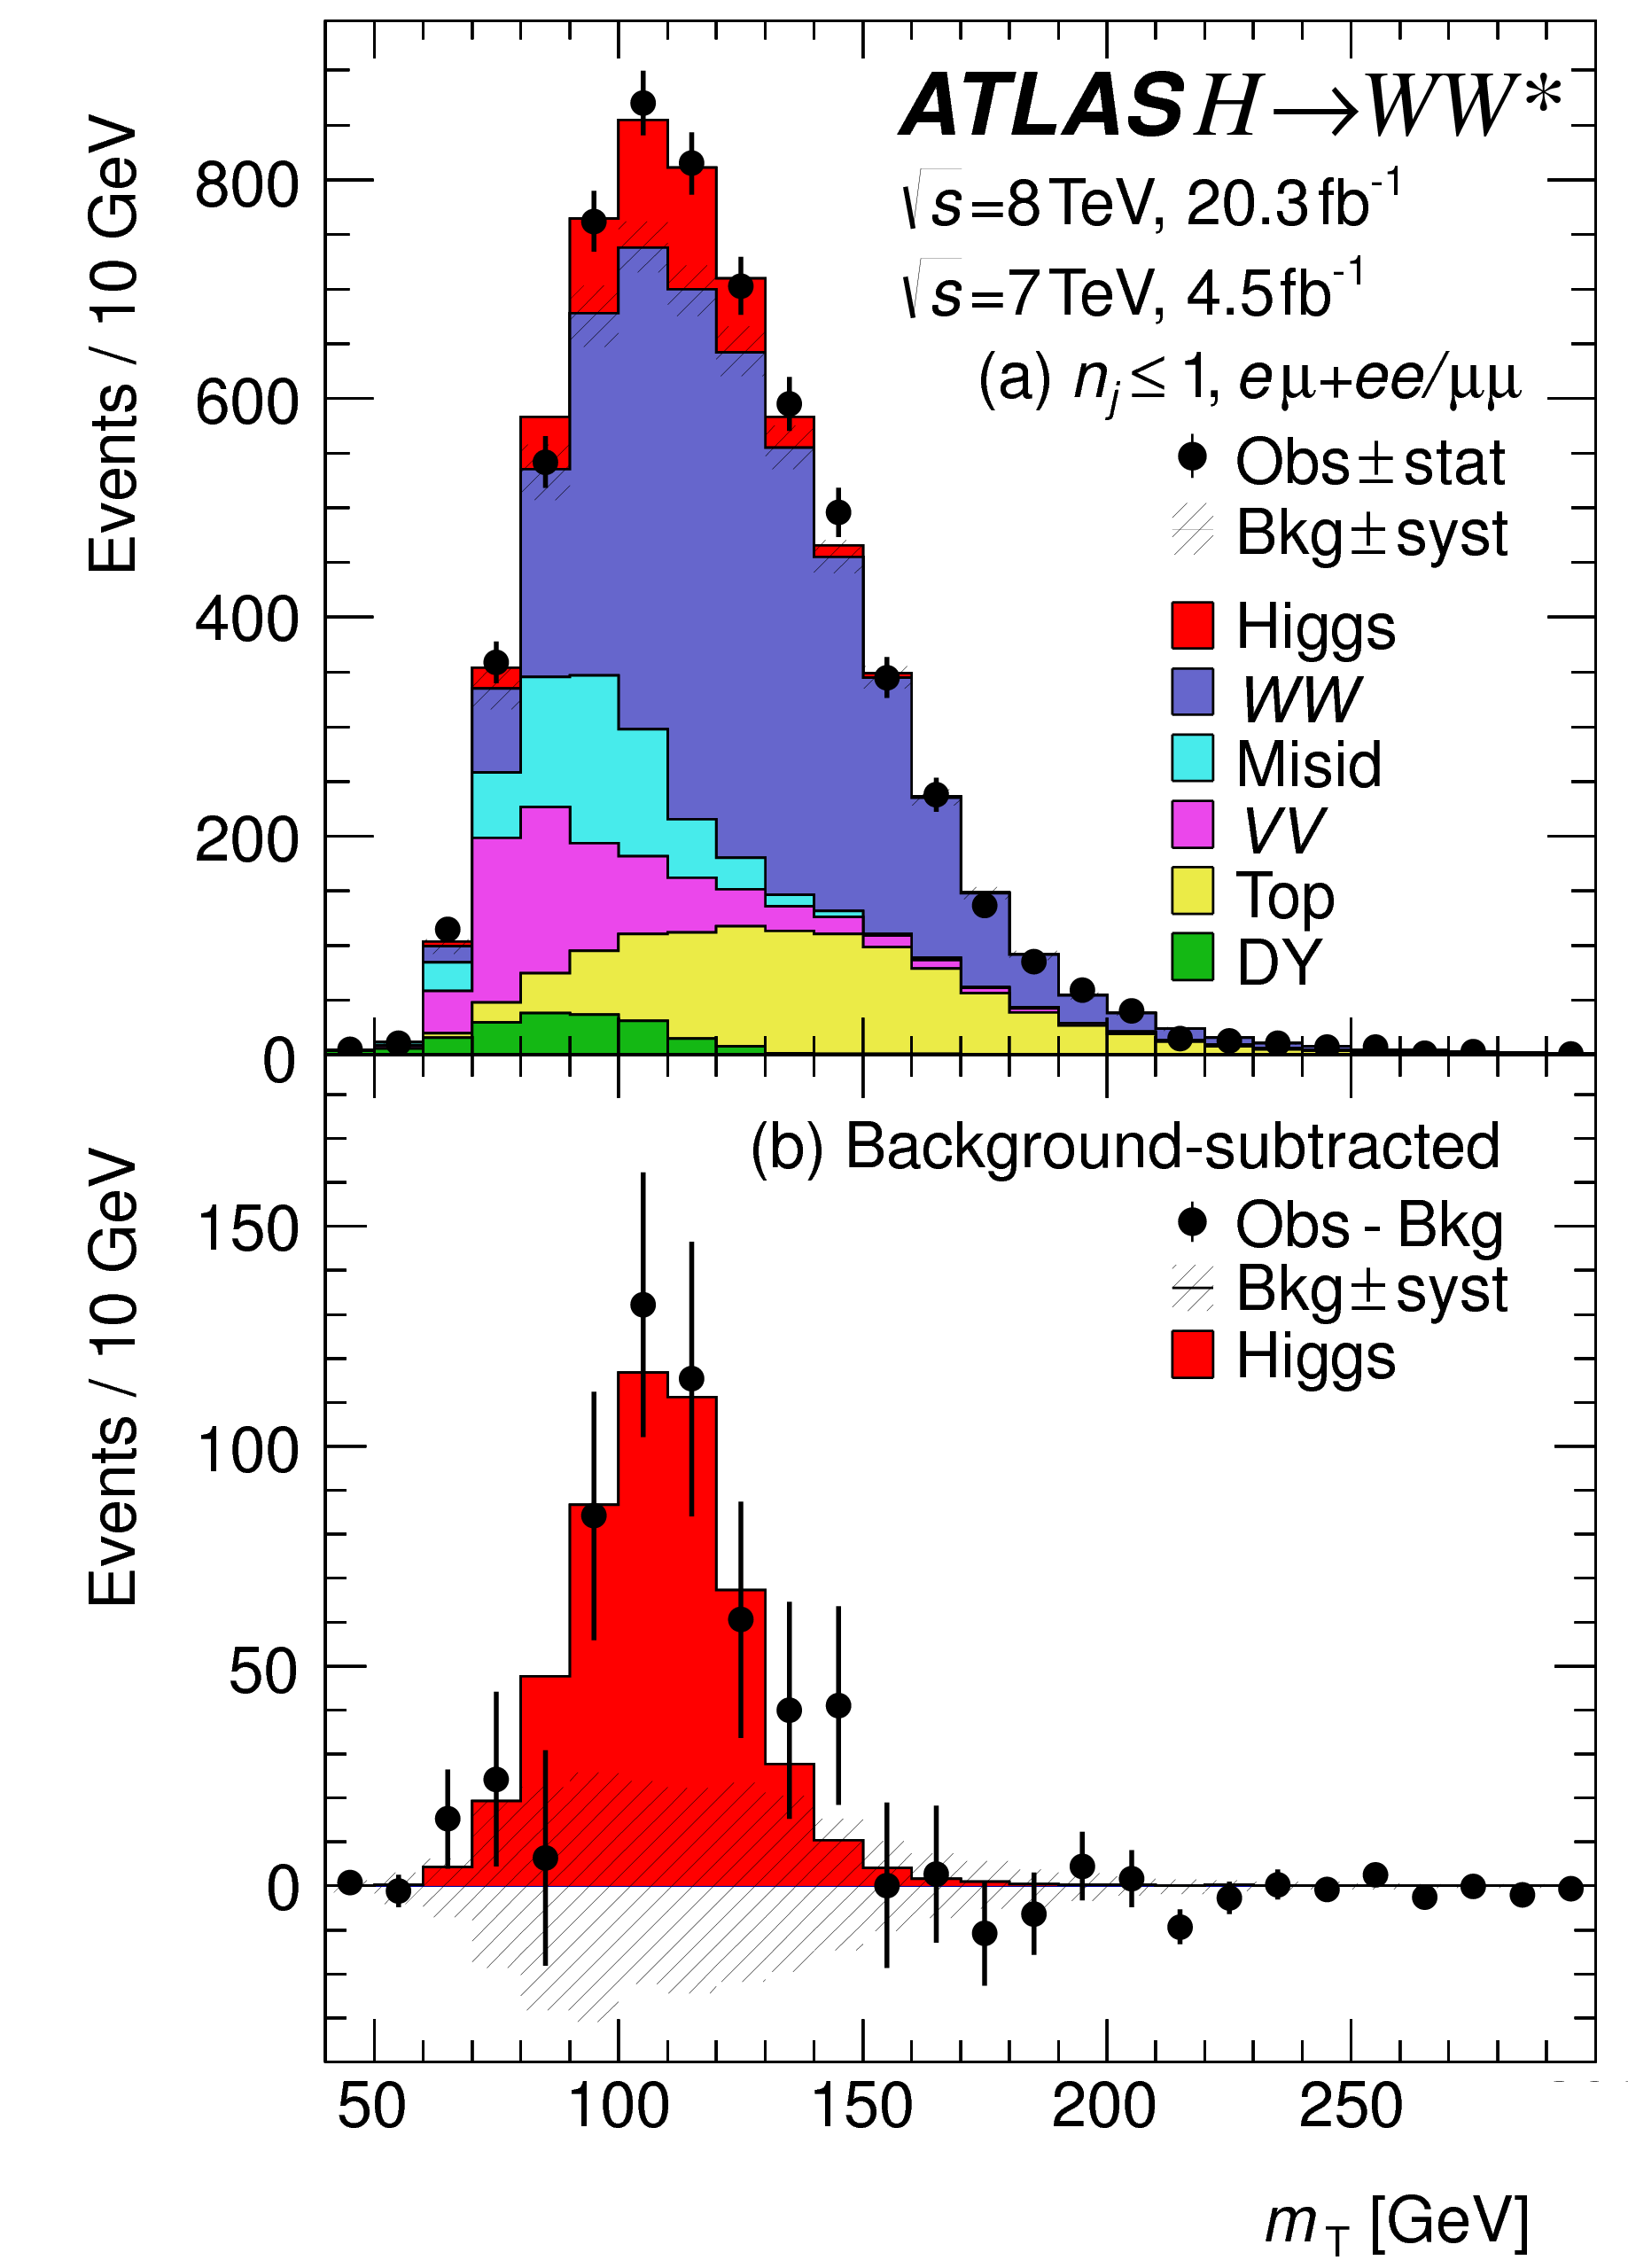
\includegraphics[width=0.6\textwidth]{figures/ggF_mT}
  \caption{Post-fit $\mTH$ distribution in the $\Njet \leq 1$ regions\cite{WW2015}.}
  \label{fig:ggF-mT}
\end{figure}

These yields are used as input, along with the VBF results in chapter 5, for the physical interpretation of results presented in subsequent sections. 

\subsection{Signal strength measurements in ggF and VBF production}

When all of the signal regions are combined in the fit, there can be a combined measurement of the signal strength as well as the individual ggF and VBF signal strengths. The combined signal strength is the ratio of the sum of the gluon fusion and VBF cross sections to the theory prediction, or a singal strength for the total Higgs production cross section that this analysis is sensitive to. The final measured combined signal strength $\mu$ is measured shown in equation~\ref{eqn:final-mu}.

\begin{equation}
\begin{array}{llllll}
 \mu
 &= 1.09%
 &^{+0.16}_{-0.15}\,(\textrm{stat.})%
 &^{+0.08}_{-0.07}\,\Big(\!\begin{tabular}{c}{\rm\footnotesize expt}\\ \noalign{\vskip -0.50truecm}{\rm\footnotesize syst}\end{tabular}\!\Big)%
 &^{+0.15}_{-0.12}\,\Big(\!\begin{tabular}{c}{\rm\footnotesize theo}\\ \noalign{\vskip -0.50truecm}{\rm\footnotesize syst}\end{tabular}\!\Big)%
 &{\PM}0.03\,\Big(\!\begin{tabular}{c}{\rm\footnotesize lumi}\\ \noalign{\vskip -0.50truecm}{\rm\footnotesize syst}\end{tabular}\!\Big)%
 \\
 \clineskip
 &= 1.09 &^{+0.16}_{-0.15}\,\textrm{(stat)} &^{+0.17}_{-0.14}\,\textrm{(syst)}
 \\
 \clineskip
 \clineskip
 &= 1.09 &^{+0.23}_{-0.21}.
\end{array}
\label{eqn:final-mu}
\end{equation}
